%%%%%%%%%%%%%%%%%%%%%%%%%%%%%%%%%%%%%%%%%
% Beamer Presentation
% LaTeX Template
% Version 1.0 (10/11/12)
%
% This template has been downloaded from:
% http://www.LaTeXTemplates.com
%
% License:
% CC BY-NC-SA 3.0 (http://creativecommons.org/licenses/by-nc-sa/3.0/)
%
%%%%%%%%%%%%%%%%%%%%%%%%%%%%%%%%%%%%%%%%%

%----------------------------------------------------------------------------------------
%	PACKAGES AND THEMES
%----------------------------------------------------------------------------------------
\documentclass{beamer}
\usepackage{tikz}
\usetikzlibrary{shapes,arrows,shadows}
\usetikzlibrary{automata,positioning,arrows}
\usepackage{amsmath,bm,times}
\usetikzlibrary{backgrounds}

\mode<presentation> {

% The Beamer class comes with a number of default slide themes
% which change the colors and layouts of slides. Below this is a list
% of all the themes, uncomment each in turn to see what they look like.

%\usetheme{default}
%\usetheme{AnnArbor}
%\usetheme{Antibes}
%\usetheme{Bergen}
\usetheme{Berkeley}
%\usetheme{Berlin}
%\usetheme{Boadilla}
%\usetheme{CambridgeUS}
%\usetheme{Copenhagen}
%\usetheme{Darmstadt}
%\usetheme{Dresden}
%\usetheme{Frankfurt}
%\usetheme{Goettingen}
%\usetheme{Hannover}
%\usetheme{Ilmenau}
%\usetheme{JuanLesPins}
%\usetheme{Luebeck}
%\usetheme{Madrid}
%\usetheme{Malmoe}
%\usetheme{Marburg}
%\usetheme{Montpellier}
%\usetheme{PaloAlto}
%\usetheme{Pittsburgh}
%\usetheme{Rochester}
%\usetheme{Singapore}
%\usetheme{Szeged}
%\usetheme{Warsaw}

% As well as themes, the Beamer class has a number of color themes
% for any slide theme. Uncomment each of these in turn to see how it
% changes the colors of your current slide theme.

%\usecolortheme{albatross}
%\usecolortheme{beaver}
%\usecolortheme{beetle}
%\usecolortheme{crane}
%\usecolortheme{dolphin}
%\usecolortheme{dove}
%\usecolortheme{fly}
%\usecolortheme{lily}
%\usecolortheme{orchid}
%\usecolortheme{rose}
%\usecolortheme{seagull}
\usecolortheme{seahorse}
%\usecolortheme{whale}
%\usecolortheme{wolverine}

%\setbeamertemplate{footline} % To remove the footer line in all slides uncomment this line
%\setbeamertemplate{footline}[page number] % To replace the footer line in all slides with a simple slide count uncomment this line

%\setbeamertemplate{navigation symbols}{} % To remove the navigation symbols from the bottom of all slides uncomment this line
}

\usepackage{graphicx} % Allows including images
\usepackage{booktabs} % Allows the use of \toprule, \midrule and \bottomrule in tables

%----------------------------------------------------------------------------------------
%	TITLE PAGE
%----------------------------------------------------------------------------------------

\title[\textsc{Scaffolding benchmarking}]{\textsc{Evaluation and benchmarking of a new scaffolding methodology}} % The short title appears at the bottom of every slide, the full title is only on the title page

\author{\textsc{Alexandrina Bodrug}} % Your name
\institute[\textsc{genscale, irisa}] % Your institution as it will appear on the bottom of every slide, may be shorthand to save space
{
\textit{\textsc{\tiny Supervisors: Pr. Rumen Andonov \& Dr. Dominique Lavenier}} \\
\vspace*{1cm}
\textsc{University Rennes 1} \\ % Your institution for the title page
\textit{\textsc{\tiny Bioinformatics and Genomics Master}} % Your email address
}
\date{\tiny \textsc{\today}} % Date, can be changed to a custom date

\begin{document}

\begin{frame}
\titlepage % Print the title page as the first slide
\end{frame}

\begin{frame}
\frametitle{Overview} % Table of contents slide, comment this block out to remove it
\tableofcontents % Throughout your presentation, if you choose to use \section{} and \subsection{} commands, these will automatically be printed on this slide as an overview of your presentation
\end{frame}

%----------------------------------------------------------------------------------------
%	PRESENTATION SLIDES
%----------------------------------------------------------------------------------------

%------------------------------------------------
\section{Context}\label{1}
\begin{frame}
\frametitle{\textsc{\nameref{1}}}
\texttt{"The \textit{Contig Scaffolding Problem}  is to order and orientate the given contigs in a manner that is consistent with as many mate-pairs as possible".}
\begin{center}
Hudson \textit{et al.} 2002
\end{center}
\end{frame}
\subsection{Some definitions}\label{2}
\begin{frame}
\frametitle{\textsc{\nameref{2}}}
\footnotesize Genome is fragmented, extremities are sequenced ($\mapsto$ reads) \ldots \\
\resizebox{7cm}{!}{
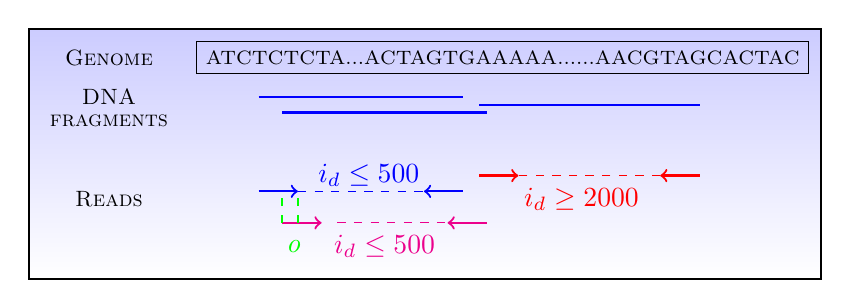
\begin{tikzpicture}[framed,background rectangle/.style={thick,draw=black, top color=blue!20}]
\node[draw=none] at (-4,0) {\footnotesize \textsc{Genome}};
\node[draw] at (1,0) {\scriptsize ATCTCTCTA...ACTAGTGAAAAA......AACGTAGCACTAC};
\node[draw=none] at (-4,-0.5) {\footnotesize \textsc{DNA}};
\node[draw=none] at (-4,-0.8) {\footnotesize \textsc{fragments}};
\draw[thick, blue] (-2.1, -0.5) -- (0.5, -0.5);
\draw[thick, blue] (0.7, -0.6) -- (3.5, -0.6);
\draw[thick, blue] (-1.8, -0.7) -- (0.8, -0.7);
\node[draw=none] at (-4,-1.8) {\footnotesize \textsc{Reads}};

\draw[red, thick, <-] (3,-1.5) -- (3.5,-1.5);
\draw[red, dashed] (3,-1.5) -- (1.2,-1.5);
\node[draw=none, color=red] at (2,-1.8) {\textit{$i_d \geq 2000$}};
\draw[red, thick, ->] (0.7,-1.5) -- (1.2,-1.5);

\draw[blue, thick, <-] (0,-1.7) -- (0.5,-1.7);
\draw[blue, dashed] (-1.6,-1.7) -- (0,-1.7);
\node[draw=none, color=blue] at (-0.7,-1.5) {\textit{$i_d\leq 500$}};
\draw[blue, thick, ->] (-2.1,-1.7) -- (-1.6,-1.7);

\draw[magenta, thick, <-] (0.3,-2.1) -- (0.8,-2.1);
\draw[magenta, dashed] (-1.1,-2.1) -- (0.3,-2.1);
\node[draw=none, color=magenta] at (-0.5,-2.4) {\textit{$i_d\leq 500$}};
\draw[magenta, thick, ->] (-1.8,-2.1) -- (-1.3,-2.1);

\node[draw=none, color=green] at (-1.65, -2.4) {\textit{o}};
\draw[green, dashed, thick] (-1.8, -2.1) -- (-1.8, -1.7); 
\draw[green, dashed, thick] (-1.6, -2.1) -- (-1.6, -1.7);
\end{tikzpicture}
}\\
\footnotesize \ldots reads are assembled though high-confidence overlappings into contigs or unitigs.\\
\resizebox{8cm}{!}{
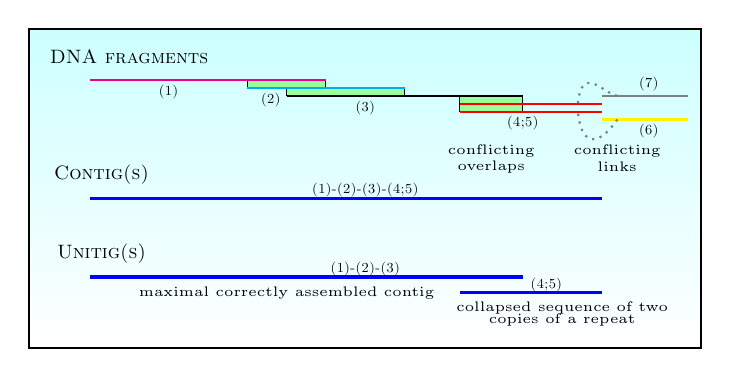
\begin{tikzpicture}[framed,background rectangle/.style={thick,draw=black, top color=cyan!20}]
\node[draw=none] at (1,0.3) {\scriptsize \textsc{DNA fragments}};
\node[draw=none] at (1.5,-0.15) {\tiny \textsc{(1)}};
\node[draw=none] at (2.8,-0.25) {\tiny \textsc{(2)}};
\node[draw=none] at (4,-0.35) {\tiny \textsc{(3)}};
\node[draw=none] at (6,-0.55) {\tiny \textsc{(4;5)}};
\node[draw=none] at (7.6,-0.65) {\tiny \textsc{(6)}};
\node[draw=none] at (7.6,-0.05) {\tiny \textsc{(7)}};
\node[draw=none] at (4,-1.4) {\tiny \textsc{(1)-(2)-(3)-(4;5)}};
\node[draw=none] at (4,-2.4) {\tiny \textsc{(1)-(2)-(3)}};
\node[draw=none] at (6.3,-2.6) {\tiny \textsc{(4;5)}};

\draw[fill=green!40] (2.5,0) -- (3.5,0) -- (3.5,-0.1) -- (2.5,-0.1) -- (2.5,0);
\draw[fill=green!40] (3,-0.1) -- (4.5,-0.1) -- (4.5,-0.2) -- (3,-0.2) -- (3,-0.1);
\draw[fill=green!40] (5.2,-0.2) -- (6.0,-0.2) -- (6.0,-0.3) -- (5.2,-0.3) -- (5.2,-0.2);
\draw[fill=green!40] (5.2,-0.3) -- (6.0,-0.3) -- (6.0,-0.4) -- (5.2,-0.4) -- (5.2,-0.3);

\draw[thick, magenta] (0.5,0) -- (3.5,0);
\draw[thick, cyan] (2.5,-0.1) -- (4.5,-0.1);
\draw[thick, black] (3.0,-0.2) -- (6.0,-0.2);
\draw[thick, red] (5.2,-0.3) -- (7,-0.3);
\draw[thick, red] (5.2,-0.4) -- (7,-0.4);
\draw[thick, yellow!] (7.0,-0.5) -- (8.1,-0.5);
\draw[thick, gray] (7.0,-0.2) -- (8.1,-0.2);

\draw[color=gray, dotted, thick] (7.2,-0.2) .. controls  (7,-0.15) and (6.75,0.2) .. (6.7,-0.3);
\draw[color=gray, dotted, thick] (7.2,-0.5) .. controls  (7,-0.8) and (6.75,-0.9) .. (6.7,-0.4);

\node[draw=none] at (5.6,-0.9) {\tiny conflicting};
\node[draw=none] at (5.6,-1.1) {\tiny overlaps};
\node[draw=none] at (7.2,-0.9) {\tiny conflicting};
\node[draw=none] at (7.2,-1.1) {\tiny links};
\node[draw=none] at (0.65,-1.2) {\scriptsize \textsc{Contig(s)}};
\draw[very thick, blue] (0.5, -1.5) -- (7, -1.5);
\node[draw=none] at (0.65,-2.2) {\scriptsize \textsc{Unitig(s)}};
\draw[very thick, blue] (0.5, -2.5) -- (6.0, -2.5);
\node[draw=none] at (3,-2.7) {\tiny maximal correctly assembled contig};
\draw[very thick, blue] (5.2, -2.7) -- (7, -2.7);
\node[draw=none] at (6.5,-2.9) {\tiny collapsed sequence of two };
\node[draw=none] at (6.5,-3.05) {\tiny copies of a repeat};
\end{tikzpicture}
}


\end{frame}
\subsection{Order and orient}\label{3}
\begin{frame}
\frametitle{\textsc{\nameref{3}}}
\resizebox{3in}{!}{
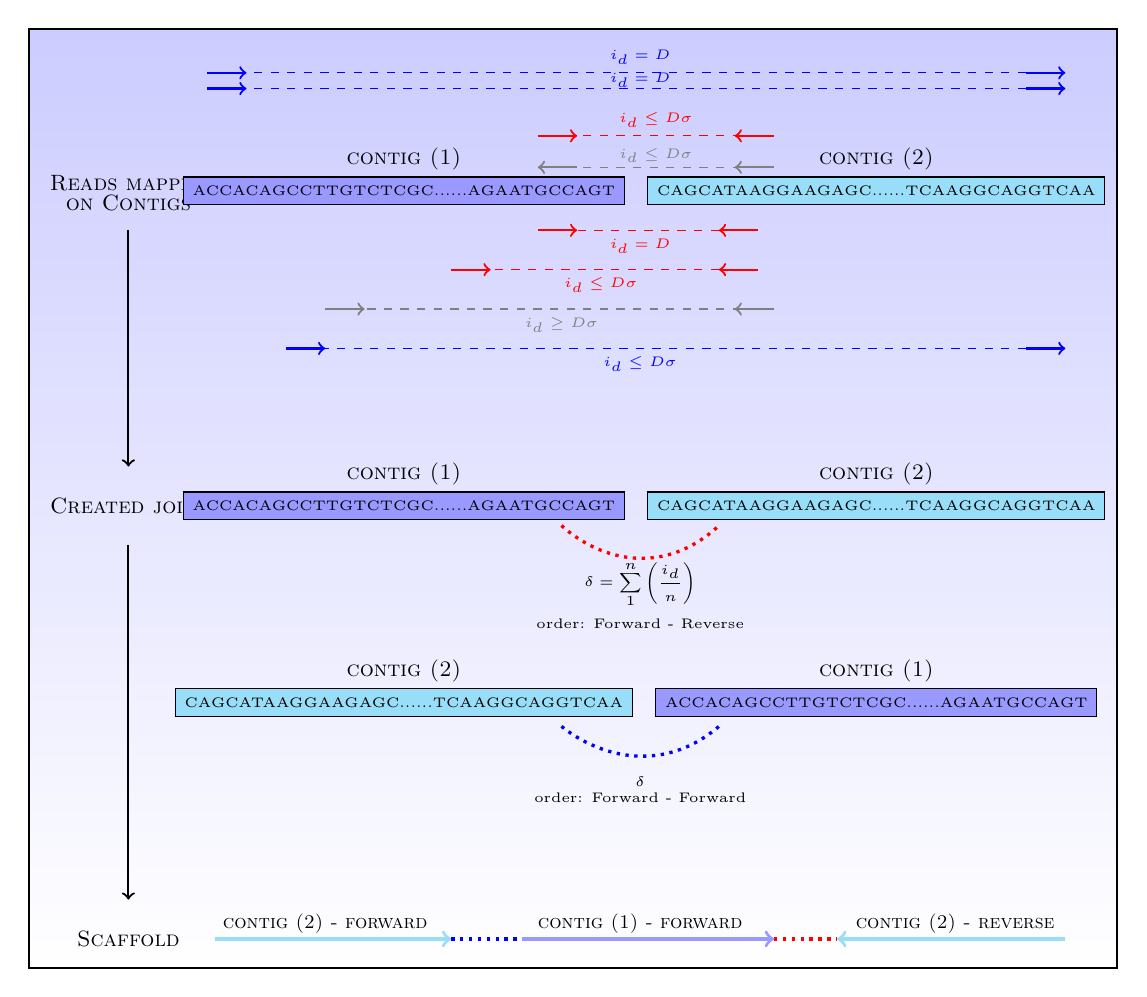
\begin{tikzpicture}[framed,background rectangle/.style={thick,draw=black, top color=blue!20}]
\node[draw=none] at (-2.5,-1.4) {\footnotesize \textsc{Reads mapped}};
\node[draw=none] at (-2.5,-1.65) {\footnotesize \textsc{on Contigs}};
\node[draw, fill=blue!40] at (1,-1.5) {\tiny ACCACAGCCTTGTCTCGC......AGAATGCCAGT};
\node[draw, fill=cyan!40] at (7,-1.5) {\tiny CAGCATAAGGAAGAGC......TCAAGGCAGGTCAA};
%red reads
\draw[red, thick, <-] (5,-2) -- (5.5,-2);
\draw[red, dashed] (5,-2) -- (3.2,-2);
\node[draw=none, color=red] at (4.0,-2.2) {\tiny {$i_d=D$}};
\draw[red, thick, ->] (2.7,-2) -- (3.2,-2);
%red reads
\draw[red, thick, <-] (5,-2.5) -- (5.5,-2.5);
\draw[red, dashed] (5,-2.5) -- (2.1,-2.5);
\node[draw=none, color=red] at (3.5,-2.7) {\tiny {$i_d\leq D\sigma$}};
\draw[red, thick, ->] (1.6,-2.5) -- (2.1,-2.5);
%red reads
\draw[red, thick, <-] (5.2,-0.8) -- (5.7,-0.8);
\draw[red, dashed] (5.7,-0.8) -- (3.2,-0.8);
\node[draw=none, color=red] at (4.2,-0.6) {\tiny {$i_d\leq D\sigma$}};
\draw[red, thick, ->] (2.7,-0.8) -- (3.2,-0.8);
%pink reads
\draw[gray, thick, <-] (5.2,-1.2) -- (5.7,-1.2);
\draw[gray, dashed] (5.7,-1.2) -- (3.2,-1.2);
\node[draw=none, color=gray] at (4.2,-1.05) {\tiny {$i_d\leq D\sigma$}};
\draw[gray, thick, ->] (3.2,-1.2) -- (2.7,-1.2);
%pink reads
\draw[gray, thick, <-] (5.2,-3) -- (5.7,-3);
\draw[gray, dashed] (5.7,-3) -- (0.5,-3);
\node[draw=none, color=gray] at (3,-3.2) {\tiny {$i_d\geq D\sigma$}};
\draw[gray, thick, ->] (0,-3) -- (0.5,-3);
%blue reads
\draw[blue, thick, <-] (9.4,0) -- (8.9,0);
\draw[blue, dashed] (8.9,0) -- (-1,0);
\node[draw=none, color=blue] at (4,0.2) {\tiny {$i_d=D$}};
\draw[blue, thick, ->] (-1.5,0) -- (-1,0);
%blue reads
\draw[blue, thick, <-] (9.4,-0.2) -- (8.9,-0.2);
\draw[blue, dashed] (8.9,-0.2) -- (-1,-0.2);
\node[draw=none, color=blue] at (4,-0.1) {\tiny {$i_d=D$ }};
\draw[blue, thick, ->] (-1.5,-0.2) -- (-1,-0.2);
%blue reads
\draw[blue, thick, <-] (9.4,-3.5) -- (8.9,-3.5);
\draw[blue, dashed] (8.9,-3.5) -- (0,-3.5);
\node[draw=none, color=blue] at (4,-3.7) {\tiny {$i_d\leq D\sigma$}};
\draw[blue, thick, ->] (-0.5,-3.5) -- (0,-3.5);
\node[draw=none] at (1,-1.1) {\footnotesize \textsc{contig (1)}};
\node[draw=none] at (7,-1.1) {\footnotesize \textsc{contig (2)}};

\begin{scope}[shift={(0,-1)}]
\node[draw=none] at (-2.5,-4.5) {\footnotesize \textsc{Created joins}};
\node[draw, fill=blue!40] at (1,-4.5) {\tiny ACCACAGCCTTGTCTCGC......AGAATGCCAGT};
\node[draw, fill=cyan!40] at (7,-4.5) {\tiny CAGCATAAGGAAGAGC......TCAAGGCAGGTCAA};
\draw[thick, ->] (-2.5, -1) -- (-2.5, -4);
\draw[color=red, dotted, very thick] (3,-4.75) .. controls  (3.5,-5.2) and (4.3,-5.4) .. (5,-4.75);
\node[draw=none] at (4,-5.5) {\tiny $\delta = \displaystyle\sum_{1}^{n}{\left(\frac{i_d}{n}\right)}$};

\node[draw=none] at (4,-6) {\tiny order: Forward - Reverse};

\node[draw, fill=cyan!40] at (1,-7) {\tiny CAGCATAAGGAAGAGC......TCAAGGCAGGTCAA};
\node[draw, fill=blue!40] at (7,-7) {\tiny ACCACAGCCTTGTCTCGC......AGAATGCCAGT};
\draw[color=blue, dotted, very thick] (3,-7.3) .. controls  (3.5,-7.7) and (4.3,-7.9) .. (5,-7.3);
\node[draw=none] at (4,-8) {\tiny $\delta$};
\node[draw=none] at (4,-8.2) {\tiny order: Forward - Forward};

\node[draw=none] at (1,-4.1) {\footnotesize \textsc{contig (1)}};
\node[draw=none] at (1,-6.6) {\footnotesize \textsc{contig (2)}};
\node[draw=none] at (7,-4.1) {\footnotesize \textsc{contig (2)}};
\node[draw=none] at (7,-6.6) {\footnotesize \textsc{contig (1)}};
%SCAFFOLD PART
\node[draw=none] at (0,-9.8) {\scriptsize \textsc{contig (2) - forward}};
\node[draw=none] at (4,-9.8) {\scriptsize \textsc{contig (1) - forward}};
\node[draw=none] at (8,-9.8) {\scriptsize \textsc{contig (2) - reverse}};
\node[draw=none] at (-2.5,-10) {\footnotesize \textsc{Scaffold}};
\draw[thick, ->] (-2.5, -5) -- (-2.5, -9.5);
\draw[very thick, ->, color=cyan!40] (-1.4,-10) -- (1.6, -10);
\draw[very thick, dotted, color=blue] (1.6,-10) -- (2.5, -10);
\draw[very thick, ->, color=blue!40] (2.5,-10) -- (5.7, -10);
\draw[very thick, dotted, color=red] (5.7,-10) -- (6.5, -10);
\draw[very thick, <-, color=cyan!40] (6.5,-10) -- (9.4, -10);
\end{scope}

\end{tikzpicture}
}
\end{frame}
\section{Genscale scaffolding tools features}\label{4}
\begin{frame}
\begin{itemize}
\item uses unitigs instead of contigs to better compute unitig coverage
\item uses unitig coverages to duplicated regions
\item several models exist, their common point is that for each unitig occurence they create a node
\item ... and for each unitig orientation, a different node is yet again created
\end{itemize}
\end{frame}
\subsection{The raw input data}\label{5}
\begin{frame}
\frametitle{\textsc{\nameref{5}}}
\textsc{Raw input data of Agrostis stolonifera} \\
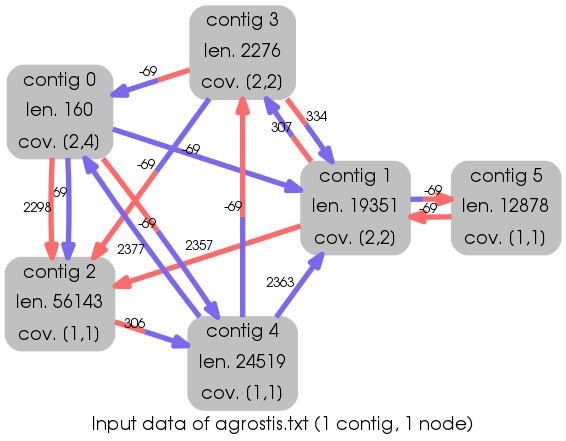
\includegraphics[scale=0.4]{agrostis_INPT_graph.png}
\end{frame}
\subsection{GST modeled graph}\label{6}
\begin{frame}
\frametitle{\textsc{\nameref{5}}}
\textsc{Graph to be solved by the GST} \\
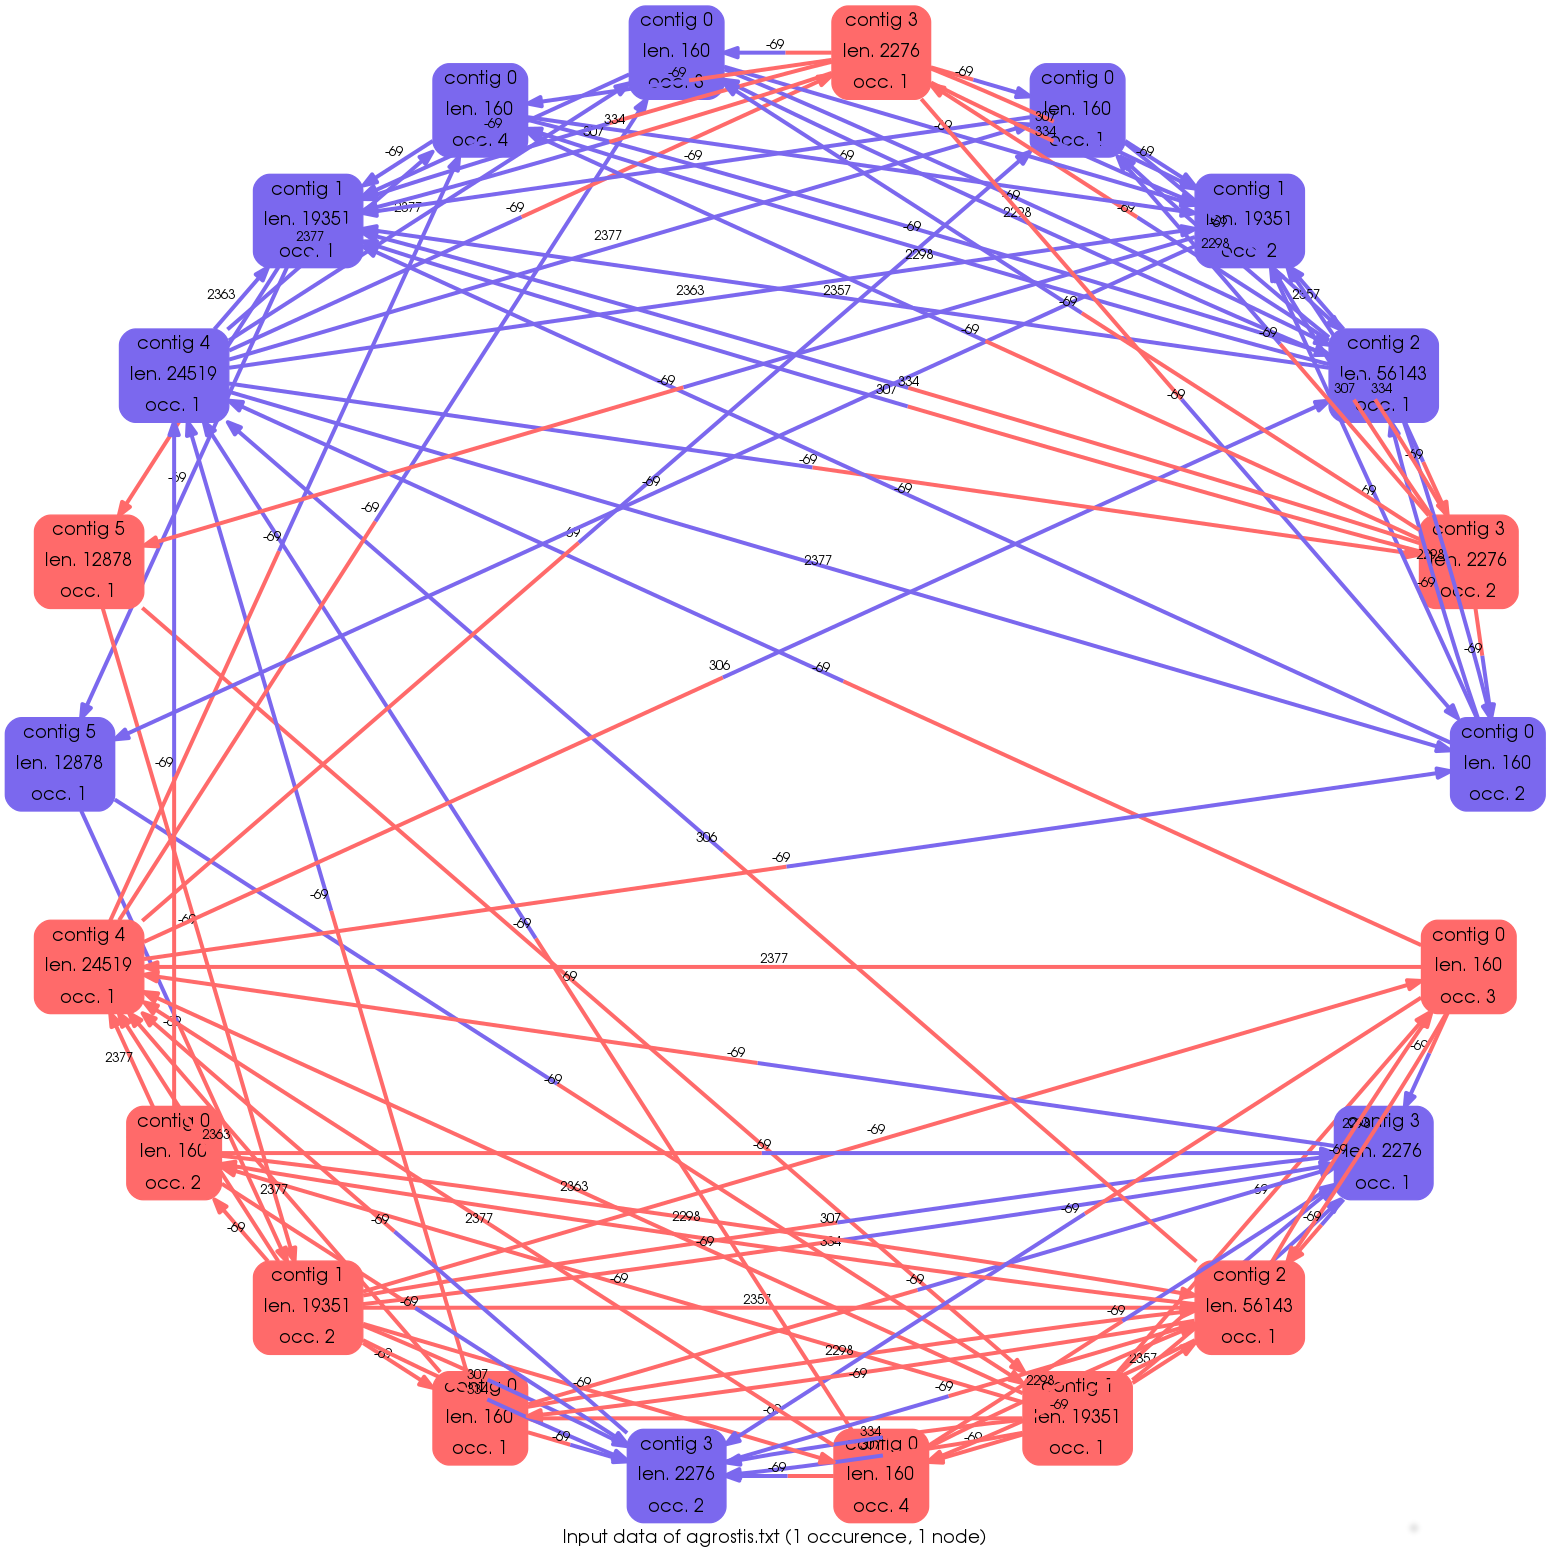
\includegraphics[scale=0.13]{agrostis_INPT_graph_model.png}
\end{frame}
\subsection{Expected solution}\label{7}
\begin{frame}
\frametitle{\textsc{\nameref{5}}}
\textsc{Expected solution of Agrostis stolonifera} \\
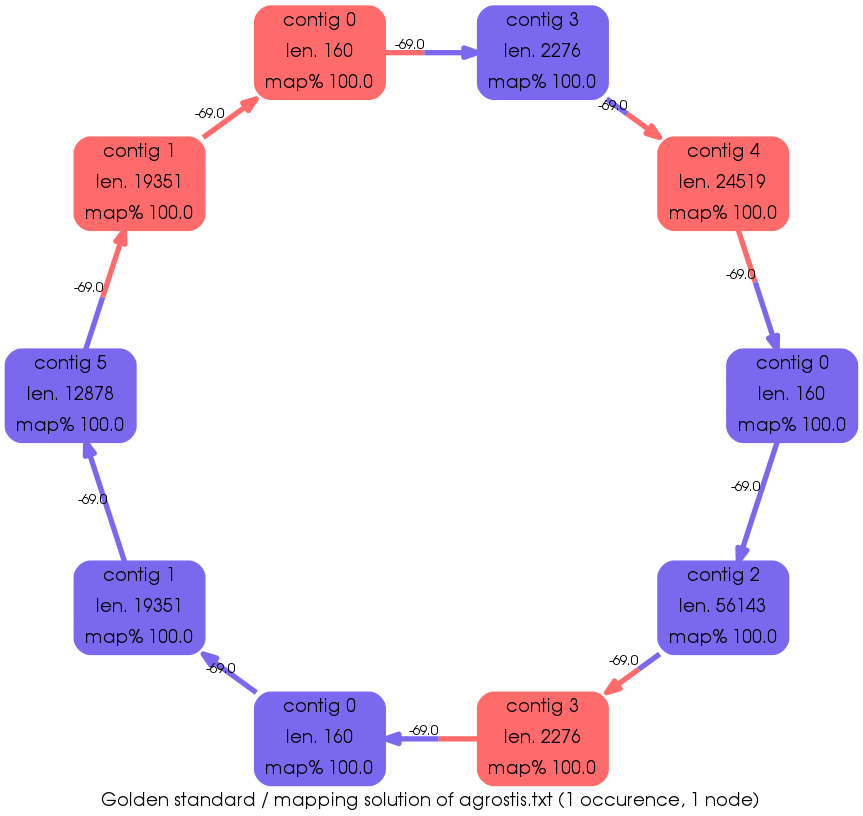
\includegraphics[scale=0.2]{agrostis_GOLD.png}
\end{frame}
\section{Challenging problem}\label{8}
\begin{frame}
\frametitle{\textsc{\nameref{8}}}
What would you do in these situations?
\resizebox{2.5in}{!}{
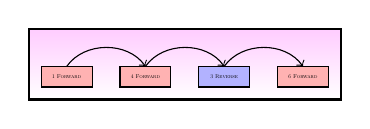
\begin{tikzpicture}[framed,background rectangle/.style={thick,draw=black, top color=magenta!20}]
\node (1F) [draw, text width=3cm, minimum height=1.3cm, fill=red!30, scale=0.2, align=center] at (0,0) {1 \textsc{Forward}};
\node (4F) [draw, text width=3cm, minimum height=1.3cm, fill=red!30, scale=0.2, align=center] at (1,0) {4 \textsc{Forward}};
\node (3R) [draw, text width=3cm, minimum height=1.3cm, fill=blue!30, scale=0.2, align=center] at (2,0) {3 \textsc{Reverse}};
\node (6F) [draw, text width=3cm, minimum height=1.3cm, fill=red!30, scale=0.2, align=center] at (3,0) {6 \textsc{Forward }};
\draw[->] (1F.north) to [bend left=55] (4F.north);
\draw[->] (4F.north) to [bend left=55] (3R.north);
\draw[->] (3R.north) to [bend left=55] (6F.north);
\end{tikzpicture}
}
\resizebox{2.5in}{!}{
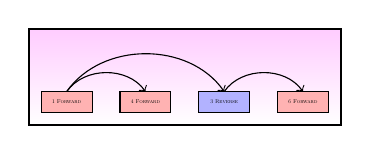
\begin{tikzpicture}[framed,background rectangle/.style={thick,draw=black, top color=magenta!20}]
\node (1F) [draw, text width=3cm, minimum height=1.3cm, fill=red!30, scale=0.2, align=center] at (0,0) {1 \textsc{Forward}};
\node (4F) [draw, text width=3cm, minimum height=1.3cm, fill=red!30, scale=0.2, align=center] at (1,0) {4 \textsc{Forward}};
\node (3R) [draw, text width=3cm, minimum height=1.3cm, fill=blue!30, scale=0.2, align=center] at (2,0) {3 \textsc{Reverse}};
\node (6F) [draw, text width=3cm, minimum height=1.3cm, fill=red!30, scale=0.2, align=center] at (3,0) {6 \textsc{Forward }};
\draw[->] (1F.north) to [bend left=55] (4F.north);
\draw[->] (1F.north) to [bend left=55] (3R.north);
%\draw[->] (4F.north) to [bend left=55] (3R.north);
\draw[->] (3R.north) to [bend left=55] (6F.north);
\end{tikzpicture}
}
\resizebox{2.5in}{!}{
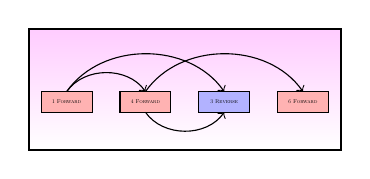
\begin{tikzpicture}[framed,background rectangle/.style={thick,draw=black, top color=magenta!20}]
\node (1F) [draw, text width=3cm, minimum height=1.3cm, fill=red!30, scale=0.2, align=center] at (0,0) {1 \textsc{Forward}};
\node (4F) [draw, text width=3cm, minimum height=1.3cm, fill=red!30, scale=0.2, align=center] at (1,0) {4 \textsc{Forward}};
\node (3R) [draw, text width=3cm, minimum height=1.3cm, fill=blue!30, scale=0.2, align=center] at (2,0) {3 \textsc{Reverse}};
\node (6F) [draw, text width=3cm, minimum height=1.3cm, fill=red!30, scale=0.2, align=center] at (3,0) {6 \textsc{Forward }};
\draw[->] (1F.north) to [bend left=55] (4F.north);
\draw[->] (1F.north) to [bend left=55] (3R.north);
\draw[->] (4F.north) to [bend left=55] (6F.north);
\draw[->] (4F.south) to [bend left=-55] (3R.south);
\end{tikzpicture}
}
\end{frame}


\section{Scripting for the GST}\label{14}
\begin{frame}
\frametitle{\textsc{\nameref{14}}}
\begin{itemize}
\item a script to visualize input data and GST solutions: \texttt{graph\_generator.py}
\item a script to inspect the features of the modeled input graph: \texttt{graph\_inspector.py}
\item a script to automatically detect correctly solved instances: \texttt{graph\_comparator.py}
\end{itemize}
\end{frame}

\section{Benchmarking workflow for tge GST}\label{9}
\begin{frame}
\frametitle{\textsc{\nameref{9}}}
\begin{figure}[h!]
\begin{center}
\resizebox{10cm}{!}{
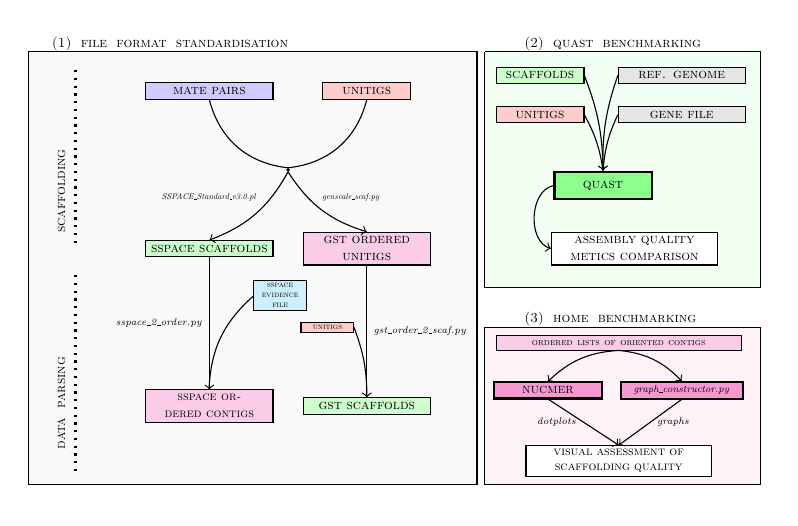
\begin{tikzpicture}
\node[text width=5cm,align=left] (filetit) [draw=none] at (0.5,0.6) {\textsc{\tiny (1) file format standardisation}};
\draw[fill=gray!5] (-2.3,0.5) -- (3.4,0.5) -- (3.4,-5) -- (-2.3,-5) -- (-2.3,0.5);
\node[text width=3cm,align=center] (mp) [draw, fill=blue!20, scale=0.5] at (0,0) {\textsc{mate pairs}};
\node[text width=2cm,align=center] (unitigs) [draw, fill=red!20, scale=0.5] at (2,0) {\textsc{unitigs}};

\node (arrowbase) [draw=none, shape=circle, fill=black, scale=0.15] at (1,-1) {};

\node[text width=3cm,align=center] (scaf) [draw, fill=green!20, scale=0.5] at (0,-2) {\textsc{sspace scaffolds}};
\node[text width=3cm,align=center] (list) [draw, fill=magenta!20, scale=0.5] at (2,-2) {\textsc{gst ordered unitigs}};

\draw (unitigs.south) to [bend left=35] (arrowbase.north);
\draw (mp.south) to [bend left=-35] (arrowbase.north);

\draw[->] (arrowbase.south) to [bend left=20] (scaf.north);
\draw[->] (arrowbase.south) to [bend right=20] (list.north);

\node[scale=0.3] (scafsspace) at (0, -1.35) {\textit{SSPACE\_Standard\_v3.0.pl}} ;
\node[scale=0.3] (scafgst) at (1.8, -1.35) {\textit{genscale\_scaf.py}} ;

\node[text width=3cm,align=center] (list2) [draw, fill=magenta!20, scale=0.5] at (0,-4) {\textsc{\small sspace ordered contigs}};
\node[text width=3cm,align=center] (scaf2) [draw, fill=green!20, scale=0.5] at (2,-4) {\textsc{gst scaffolds}};

\draw [->] (scaf.south) -- node[scale=0.7, left] {\tiny \textit{sspace\_2\_order.py}} (list2.north);
\draw [->] (list.south) -- node[scale=0.7, right] {\tiny \textit{gst\_order\_2\_scaf.py}} (scaf2.north);

\node[text width=2cm,align=center] (evidence) [draw, fill=cyan!20, scale=0.3] at (0.9,-2.6) {\textsc{sspace evidence file}};
\draw (evidence.west) to [bend right=23] (list2);

\node[text width=2cm,align=center] (unitigsbis) [draw, fill=red!20, scale=0.3] at (1.5,-3) {\textsc{unitigs}};
\draw (unitigsbis.east) to [bend left=10] (scaf2);

%somearrows
\node (A) [draw=none, shape=circle] at (-1.7,0.5) {};
\node (B) [draw=none, shape=circle] at (-1.7,-2.1) {};
\node (C) [draw=none, shape=circle] at (-1.7,-5) {};

\draw[sloped, anchor=center, above, text width=2.0cm, thick, dotted] (B) -- node{\tiny \textsc{scaffolding}} (A);


\draw[sloped, anchor=center, above, text width=2.0cm,thick, dotted] (C) -- node{\tiny \textsc{data parsing}}(B);

%benchmarking titles
\node[text width=3cm,align=left] (quasttit) [draw=none] at (5.5,0.6) {\textsc{\tiny (2) quast benchmarking}};
\node[text width=3cm,align=left] (hometit) [draw=none] at (5.5,-2.9) {\textsc{\tiny (3) home benchmarking}};
\draw[fill=green!5] (3.5,0.5) -- (7,0.5) -- (7,-2.5) -- (3.5,-2.5) -- (3.5,0.5);
\draw[fill=magenta!5] (3.5,-3) -- (7,-3) -- (7,-5) -- (3.5,-5) -- (3.5,-3);
%benchmarking quast guts
\node[text width=2cm,align=center] (scafs) [draw, fill=green!20, scale=0.5] at (4.2,0.2) {\textsc{scaffolds}};
\node[text width=2cm,align=center] (unitigs) [draw, fill=red!20, scale=0.5] at (4.2,-0.3) {\textsc{unitigs}};
\node[text width=3cm,align=center] (refgenome) [draw, fill=gray!20, scale=0.5] at (6,0.2) {\textsc{ref. genome}};
\node[text width=3cm,align=center] (gfile) [draw, fill=gray!20, scale=0.5] at (6,-0.3) {\textsc{gene file}};
\node[text width=1cm, align=center] (quastbam) [draw, thick, fill=green!45] at (5,-1.2) {\textsc{\tiny quast}};
\draw[thin, ->] (scafs.east) to [bend left=10] (quastbam.north);
\draw[thin, ->] (refgenome.west) to [bend left=-10] (quastbam.north);
\draw[thin] (unitigs.east) to [bend left=10] (quastbam.north);
\draw[thin] (gfile.west) to [bend left=-10] (quastbam.north);
\node[text width=4cm, align=center] (metrics) [draw, fill=white, scale=0.5] at (5.4,-2) {\textsc{assembly quality metics comparison}};
\draw[thin, ->] (quastbam.west) to [bend left=-75] (metrics.west);
%benchmarking home guts
\node[text width=6cm,align=center] (orders) [draw, fill=magenta!20, scale=0.5] at (5.2,-3.2) {\textsc{\scriptsize ordered lists of oriented contigs}};
\node[text width=2.5cm,align=center] (mummer) [draw, thick, fill=magenta!40, scale=0.5] at (4.3,-3.8) {\textsc{nucmer}};
\node[text width=3.2cm,align=center] (constructor) [draw, thick, fill=magenta!40, scale=0.45] at (6,-3.8) {\textit{\footnotesize graph\_constructor.py}};

\draw[thin, ->] (orders.south) to [bend left=-20] (mummer.north);
\draw[thin, ->] (orders.south) to [bend left=20] (constructor.north);

\node[text width=5cm,align=center] (viz) [draw, fill=white, scale=0.45] at (5.2,-4.7) {\textsc{visual assessment of scaffolding quality}};

\draw [->] (mummer.south) -- node[scale=0.7, left] {\tiny \textit{dotplots}} (viz.north);
\draw [->] (constructor.south) -- node[scale=0.7, right] {\tiny \textit{graphs}} (viz.north);
\end{tikzpicture}
}
\end{center}
\caption{Benchmarking workflow}
\label{fig:benchwork}
\end{figure}
\end{frame}

\section{Results}\label{15}
\begin{frame}
\frametitle{\textsc{\nameref{15}}}
\begin{itemize}
\item Genomes with big repeated regions were solved a lot better than SSPACE
\item Small repeats are very challenging to assemble because too many conflicting links exists and GST can not take a decision or is too slow
\end{itemize}
\end{frame}

\subsection{Example of Agrostis stolonifera}\label{16}
\begin{frame}
\frametitle{\textsc{\nameref{16}}}
\begin{figure}[h!]
\begin{center}
\resizebox{9cm}{!}{
\begin{tikzpicture}
\node (wpm1) at (0,0) {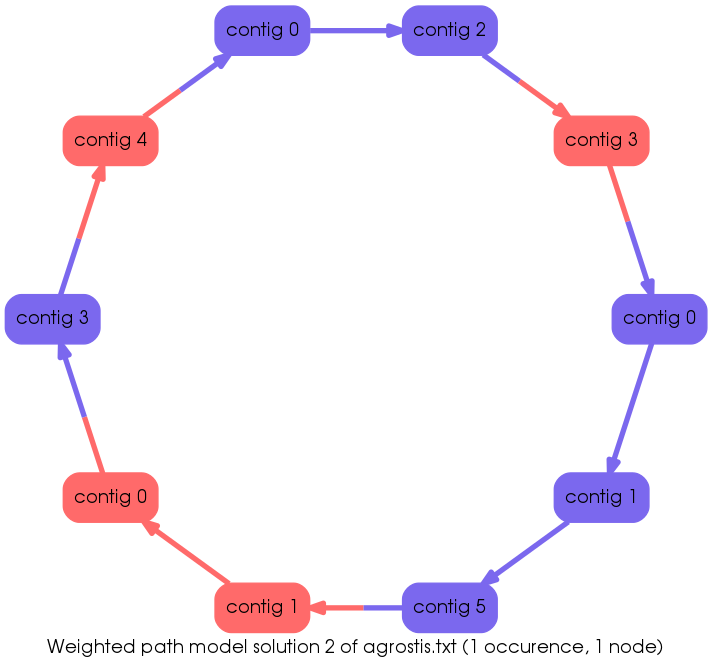
\includegraphics[scale=0.25]{wpm_agrostis_sol1}};
\node (wmp2) at (8,0) {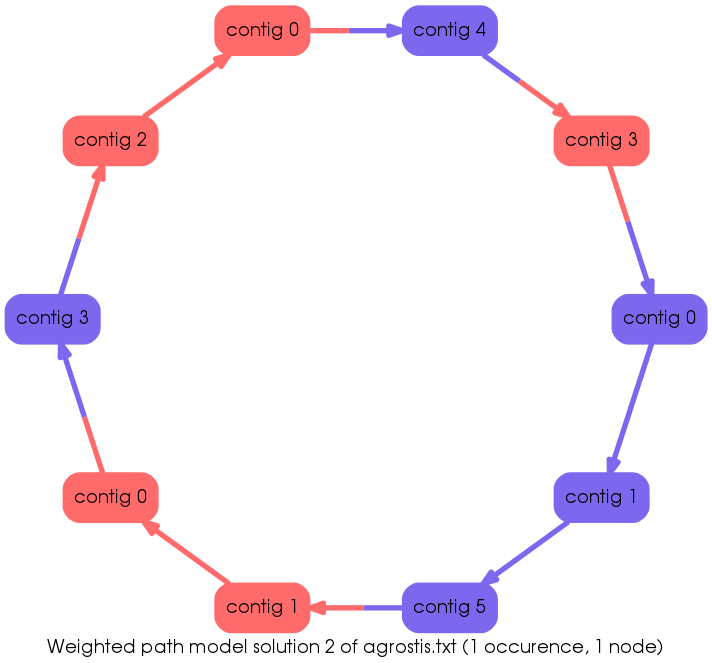
\includegraphics[scale=0.25]{wpm_agrosti_sol2}};
\node (sspace) at (9,7) {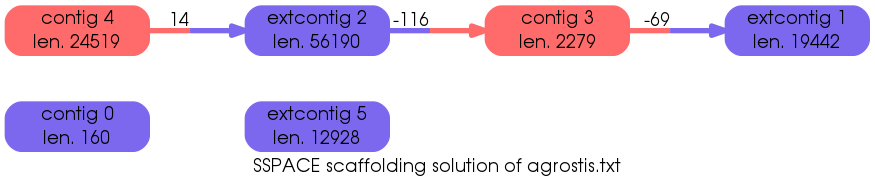
\includegraphics[scale=0.25]{sspace_scaffolds_agrostis}};
\node (gold) at (0,7) {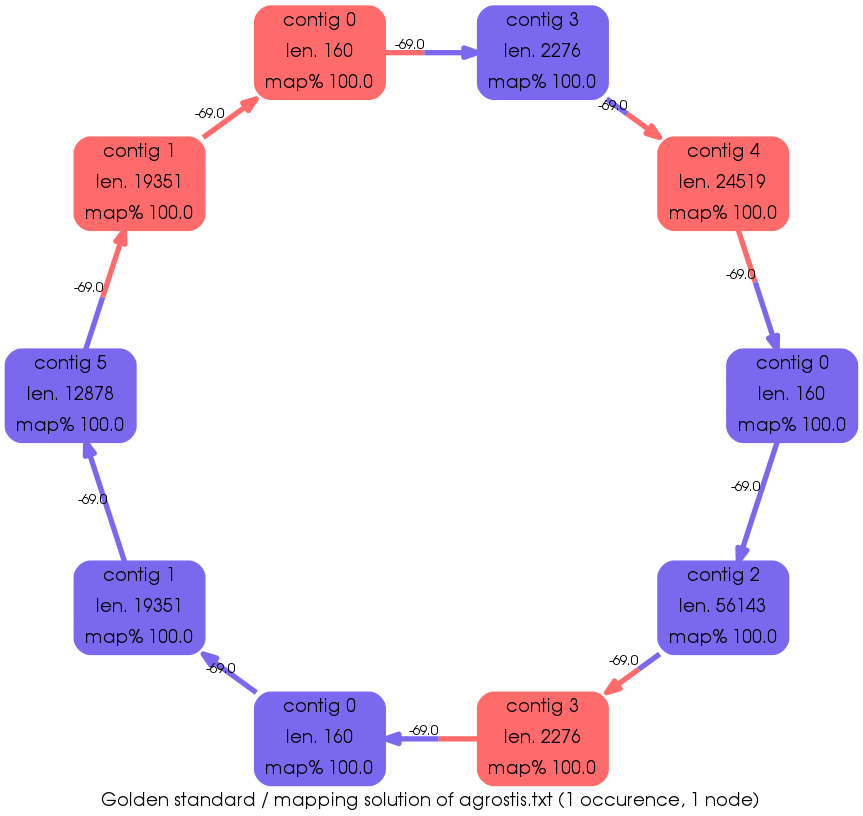
\includegraphics[scale=0.25]{agrostis_GOLD}};

\draw [blue!30,ultra thick,domain=-30:40] plot ({3.3*cos(\x)}, {3.3*sin(\x)});
\draw [blue!30,ultra thick,domain=175:255] plot ({3.3*cos(\x)}, {3.3*sin(\x)});
\begin{scope}[shift={(8,0)}]
\draw [blue!30,ultra thick,domain=-30:40] plot ({3.3*cos(\x)}, {3.3*sin(\x)});
\draw [blue!30,ultra thick,domain=175:255] plot ({3.3*cos(\x)}, {3.3*sin(\x)});
\end{scope}
\begin{scope}[shift={(0,7.1)}]
\draw [blue!30,ultra thick,domain=70:150] plot ({3.9*cos(\x)}, {3.9*sin(\x)});
\draw [blue!30,ultra thick,domain=210:290] plot ({3.9*cos(\x)}, {3.9*sin(\x)});
\end{scope}
\begin{scope}[shift={(11,7.5)}]
\draw [blue!30,ultra thick,domain=0:360] plot ({2*cos(\x)}, {1*sin(\x)});
\end{scope}
\begin{scope}[shift={(5.9,6.7)}]
\draw [blue!30,ultra thick,domain=0:360] plot ({1*cos(\x)}, {0.5*sin(\x)});
\end{scope}

\end{tikzpicture}
}
\end{center}
\caption{Expected solution and scaffolding solutions of weighted-path model and SSPACE scaffolders}

\label{fig:scafsols}
\end{figure}
\end{frame}

\section{Perspectives}\label{17}
\begin{frame}
\frametitle{\textsc{\nameref{17}}}
\begin{itemize}
\item Find strategies which solve more challenging data (flow model)
\item Scaffold bacterial data
\item Test the GST with real data
\end{itemize}
\end{frame}

\begin{frame}
\Huge{{ Thanks! \\ \vspace*{2cm} The End}}
\end{frame}
%----------------------------------------------------------------------------------------

\end{document} 